%%%%%%%%%%%%%%%%%%%%%%%%%%%%%%%%%%%%%%%%%%%%%%
%                insertmeeting
% 1) Title (something creative & funny?)
% 2) Date (MM/DD/YYYY)
% 3) Location (ex. Hagerty High School)
% 4) People/Committees Present 
% 5) Picture 
% 6) Start Time & Stop Time (ex. 12:30AM to 4:30PM)
%%%%%%%%%%%%%%%%%%%%%%%%%%%%%%%%%%%%%%%%%%%%%%
\insertmeeting 
	{Updating FLL Junior Website} 
	{09/16/21}
	{Hagerty High School}
	{Annika, Falon, Rose}
	{Images/RobotPics/robot.jpg}
	{2:30 - 4:30}
	
\subsection*{Multimedia}
\noindent\hfil\rule{\textwidth}{.4pt}\hfil
\subsubsection*{Goals}
\begin{itemize}
    \item Update the FLL Jr. website.

\end{itemize} 

\noindent\hfil\rule{\textwidth}{.4pt}\hfil

\subsubsection*{Accomplishments}
Today we worked on updating the FLL website for the current season of Cargo Connect to ensure communication with our community. Falon, Annika, and Rose added more pages to the website, and updated the team names and numbers. We also updated photos for the mentors and have established a section for the members. Next, we will focus on taking team photos of the FLL kids at the next meeting (September, Friday the 17th).

\begin{figure}[htp]
\centering
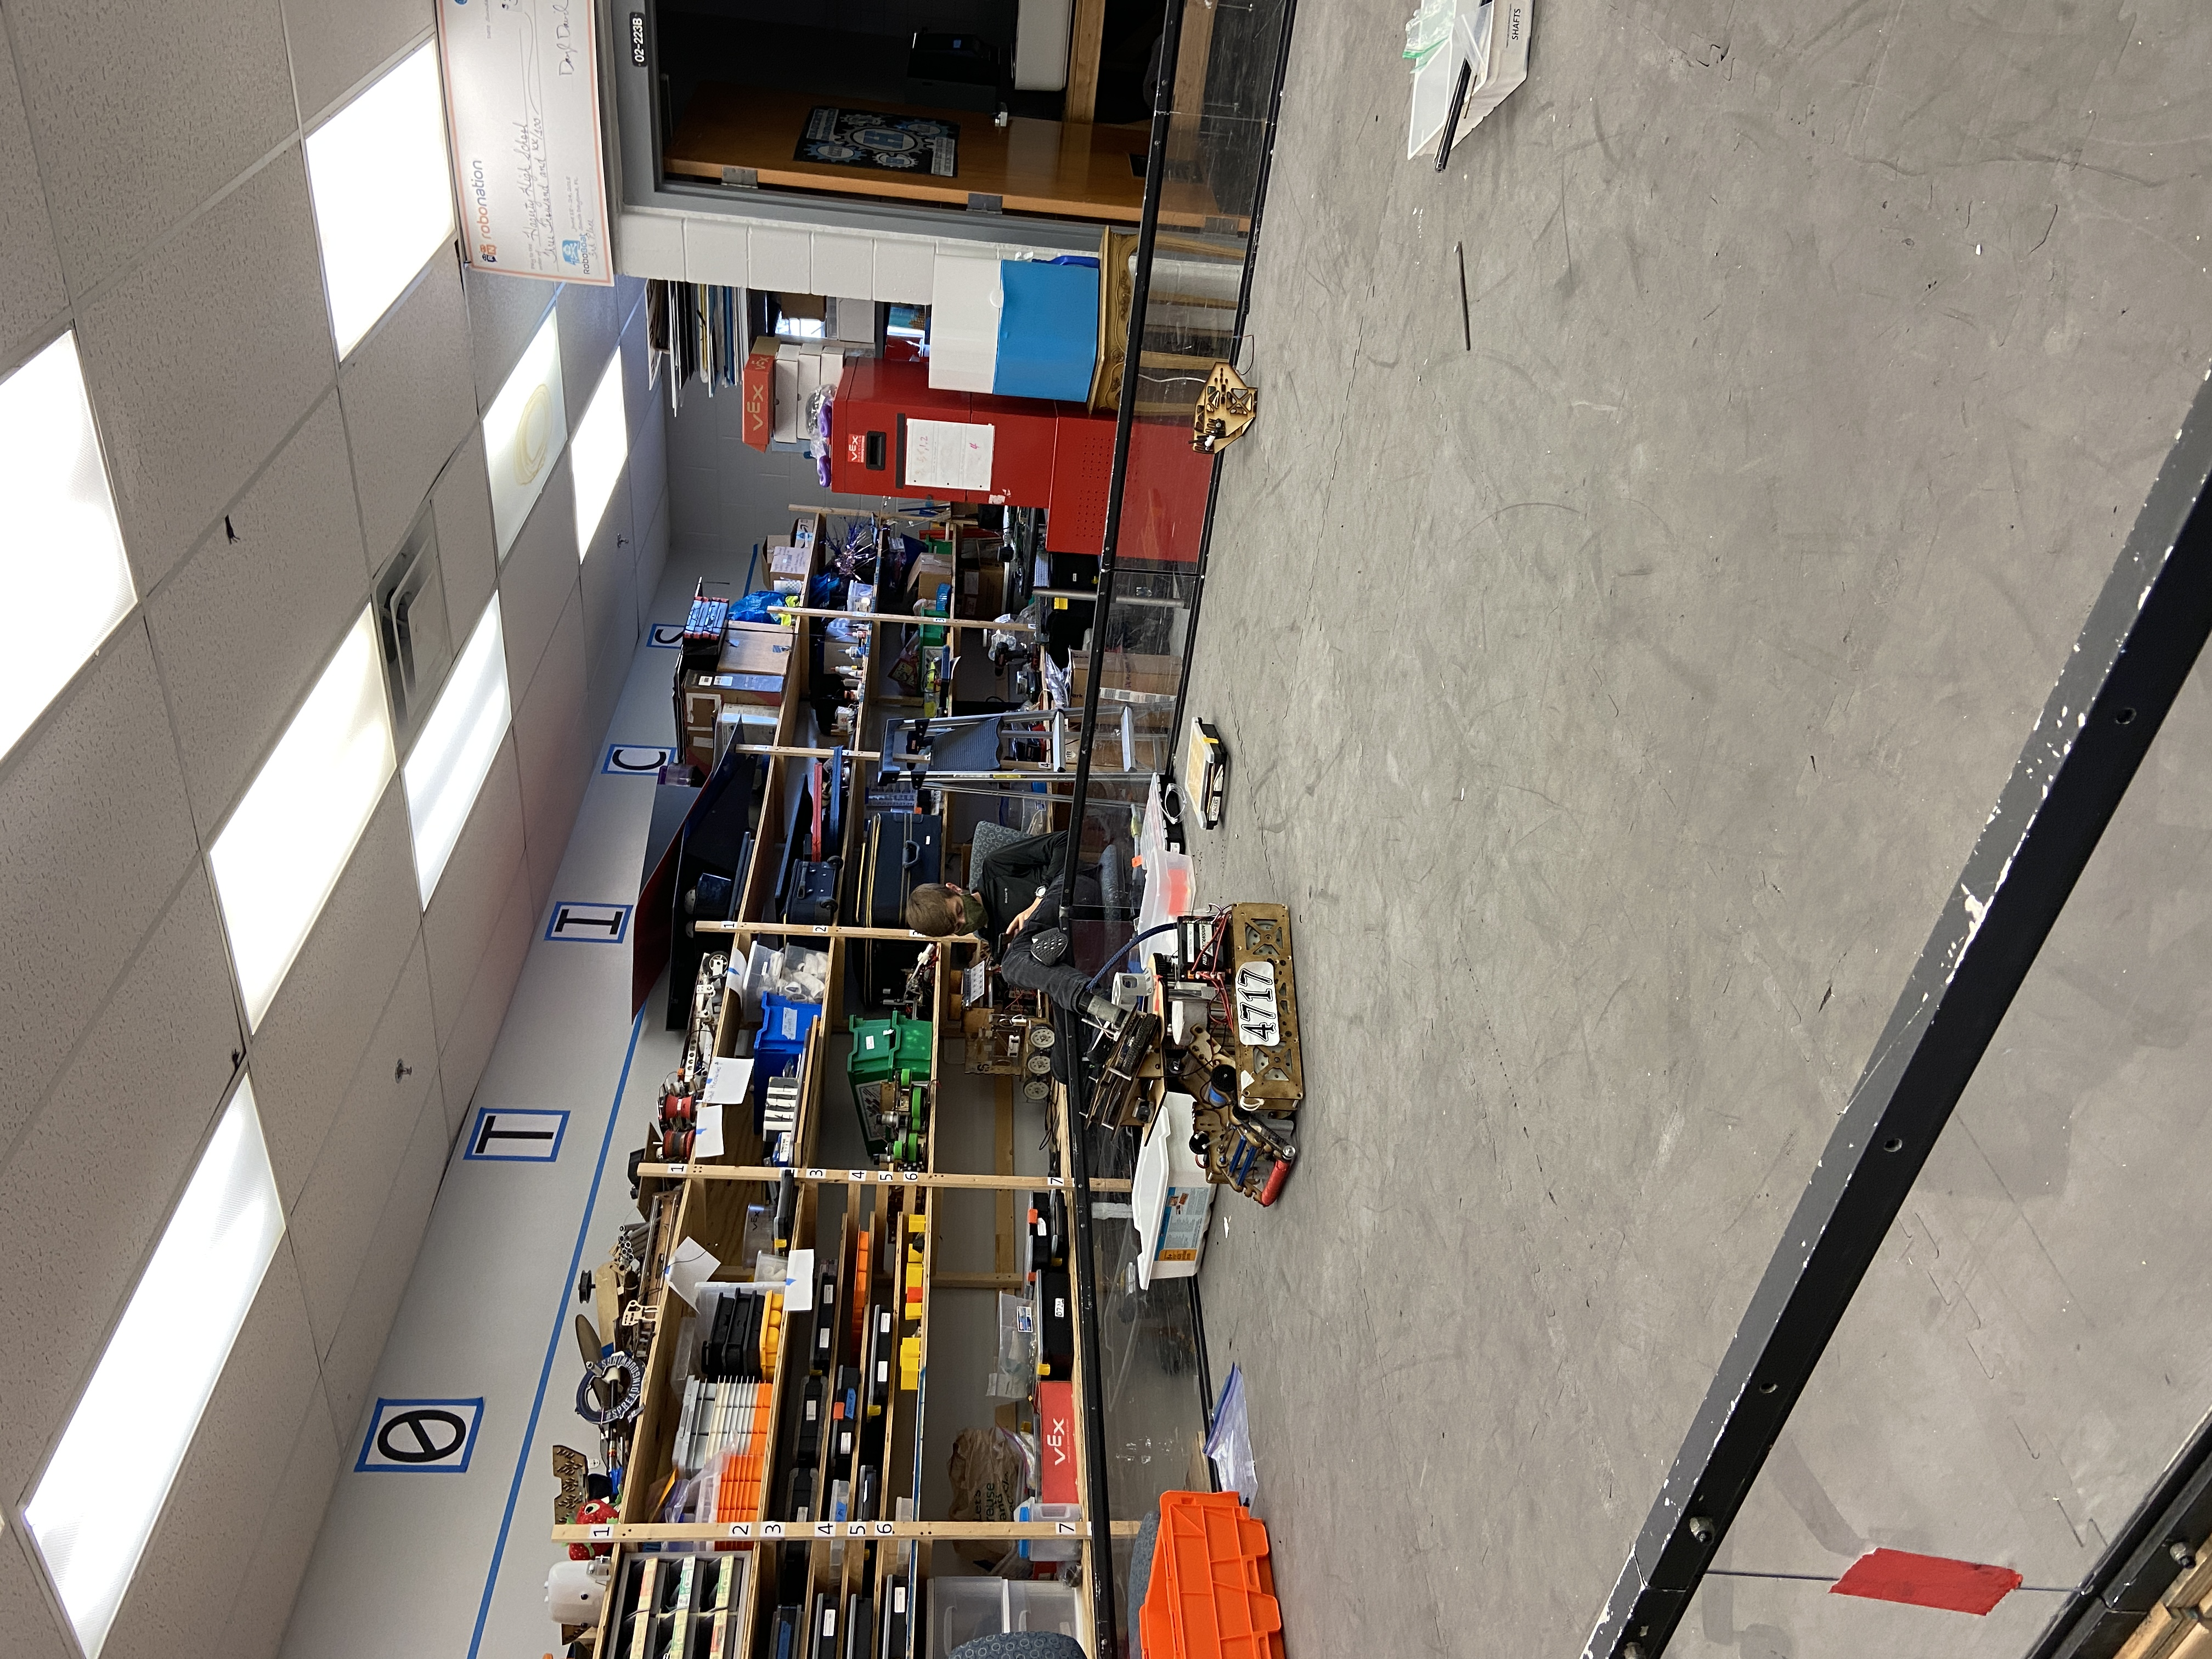
\includegraphics[width=0.9\textwidth, angle=0]{Meetings/September/09-16-21/IMG_8833 - Falon Jones.JPG}
\caption{Jensen writing notebook entries after meeting the FLL kids.}
\label{fig:pic1}
\end{figure}

\subsection*{Hardware}
\noindent\hfil\rule{\textwidth}{.4pt}\hfil
\subsubsection*{Goals}
\begin{itemize}
    \item fix belt issues on mecanum drivetrain
	\item Fix shaft issues on mecanum drivetrain

\end{itemize} 

\noindent\hfil\rule{\textwidth}{.4pt}\hfil

\subsubsection*{Accomplishments}
As we continued to work with our mecanum drivetrain, we found that the edges of the mecanum wheels were hitting the belts at some points (image 1). This is an issue because over time, the belts might be damaged, and the friction from the wheels hitting the belt might slow down one of the wheels, preventing the robot from driving straight. In addition to the wheels hitting the belts, we found that some of the shafts for the wheels were too short and led to the bearings falling out (image 2). If this were to happen during the match, our robot would be unable to move around the field effectively. To fix both of these issues, we are redesigning some parts of the drivetrain. To prevent the wheels from hitting the belts, we changed the cad of the wheel pulley, designing it to stick out 0.1 inch farther from the wheel, providing the clearance we need without expanding the drivetrain too much (image 3). This means that we will need to take the entire wheel assembly apart and reprint the pulleys, then rebuild the entire assembly. While we are putting everything back together, we will swap out the short shafts for longer ones that we will buy and cut to the right length. This should fix all of the issues we have found with the drivetrain of our mecanum drive, and will give us a smoother start to the season, once the game comes out. In the future we'll focus on printing new wheel pulleys,
buying and cutting new shafts to the right length, and 
rebuildling wheel assemblies with new pulleys and shafts.



\begin{figure}[ht]
\centering
\begin{minipage}[b]{.50\textwidth}
  \centering
  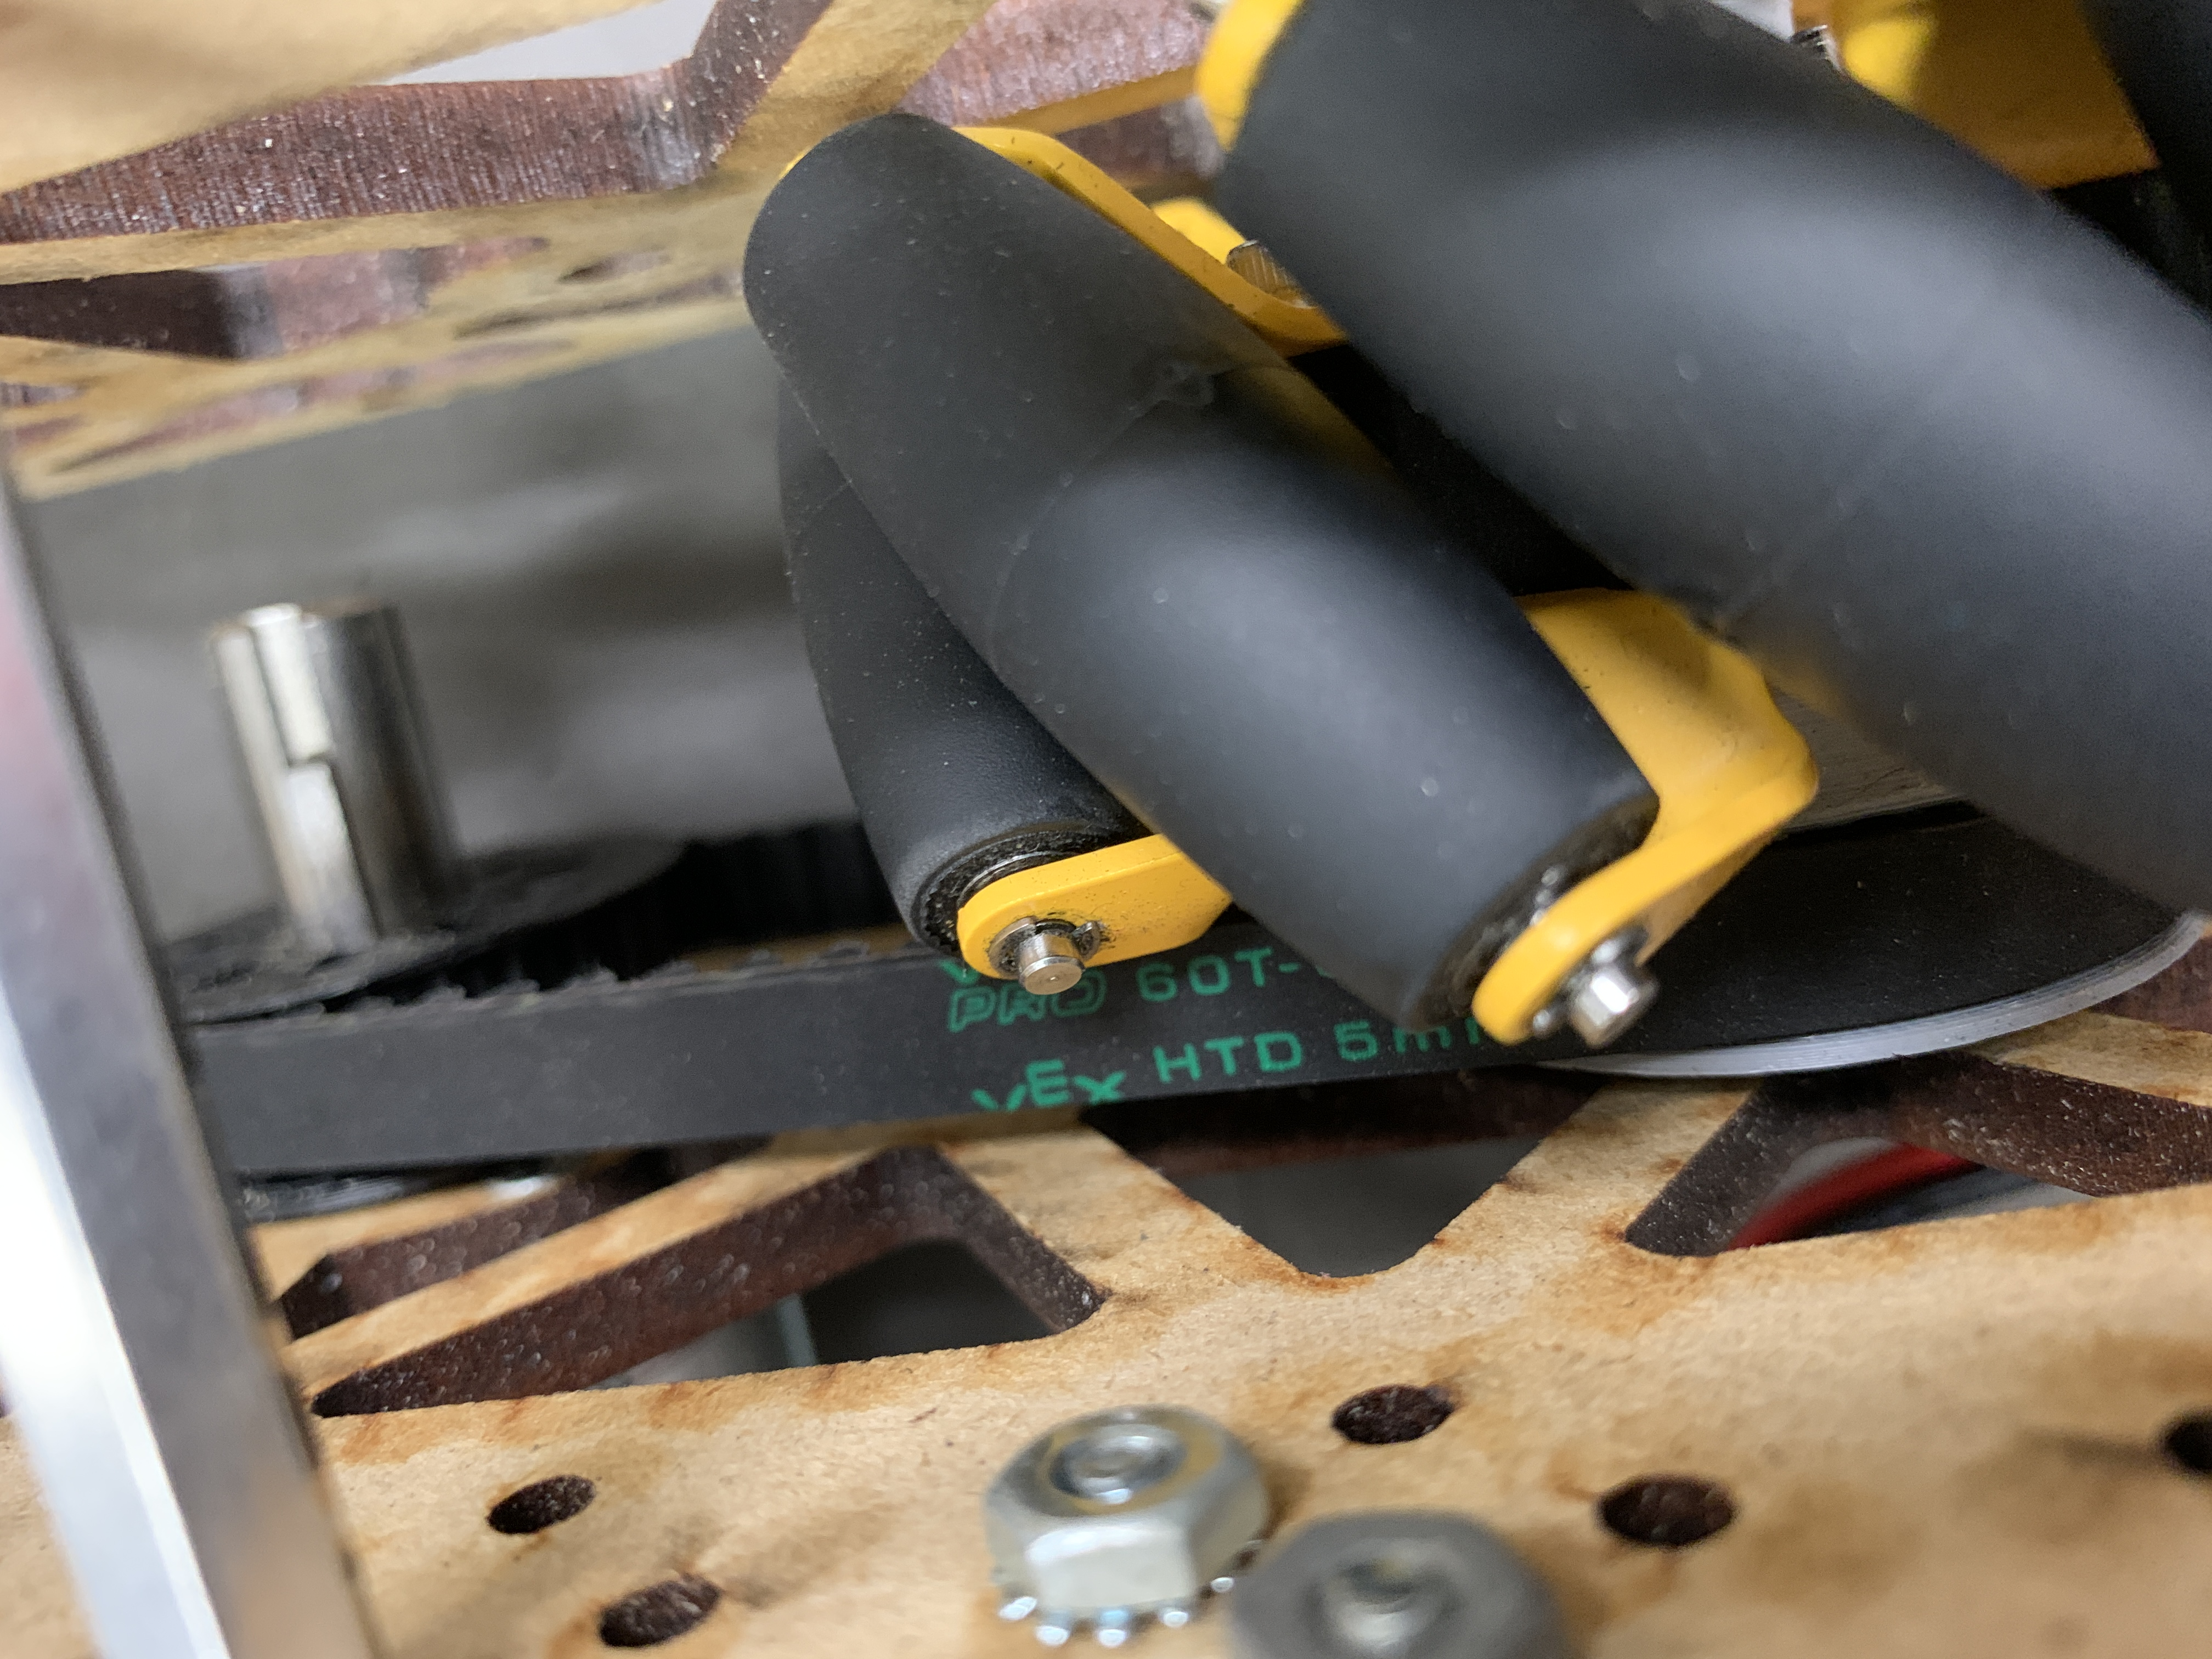
\includegraphics[width=0.8\textwidth]{Meetings/September/09-16-21/9-16-21_Hardware_Image1 - Nathan Forrer.JPG}
  \caption{The belts detailed in the entry.}
  \label{fig:pic1}
\end{minipage}%
\hfill%
\begin{minipage}[b]{.50\textwidth}
  \centering
  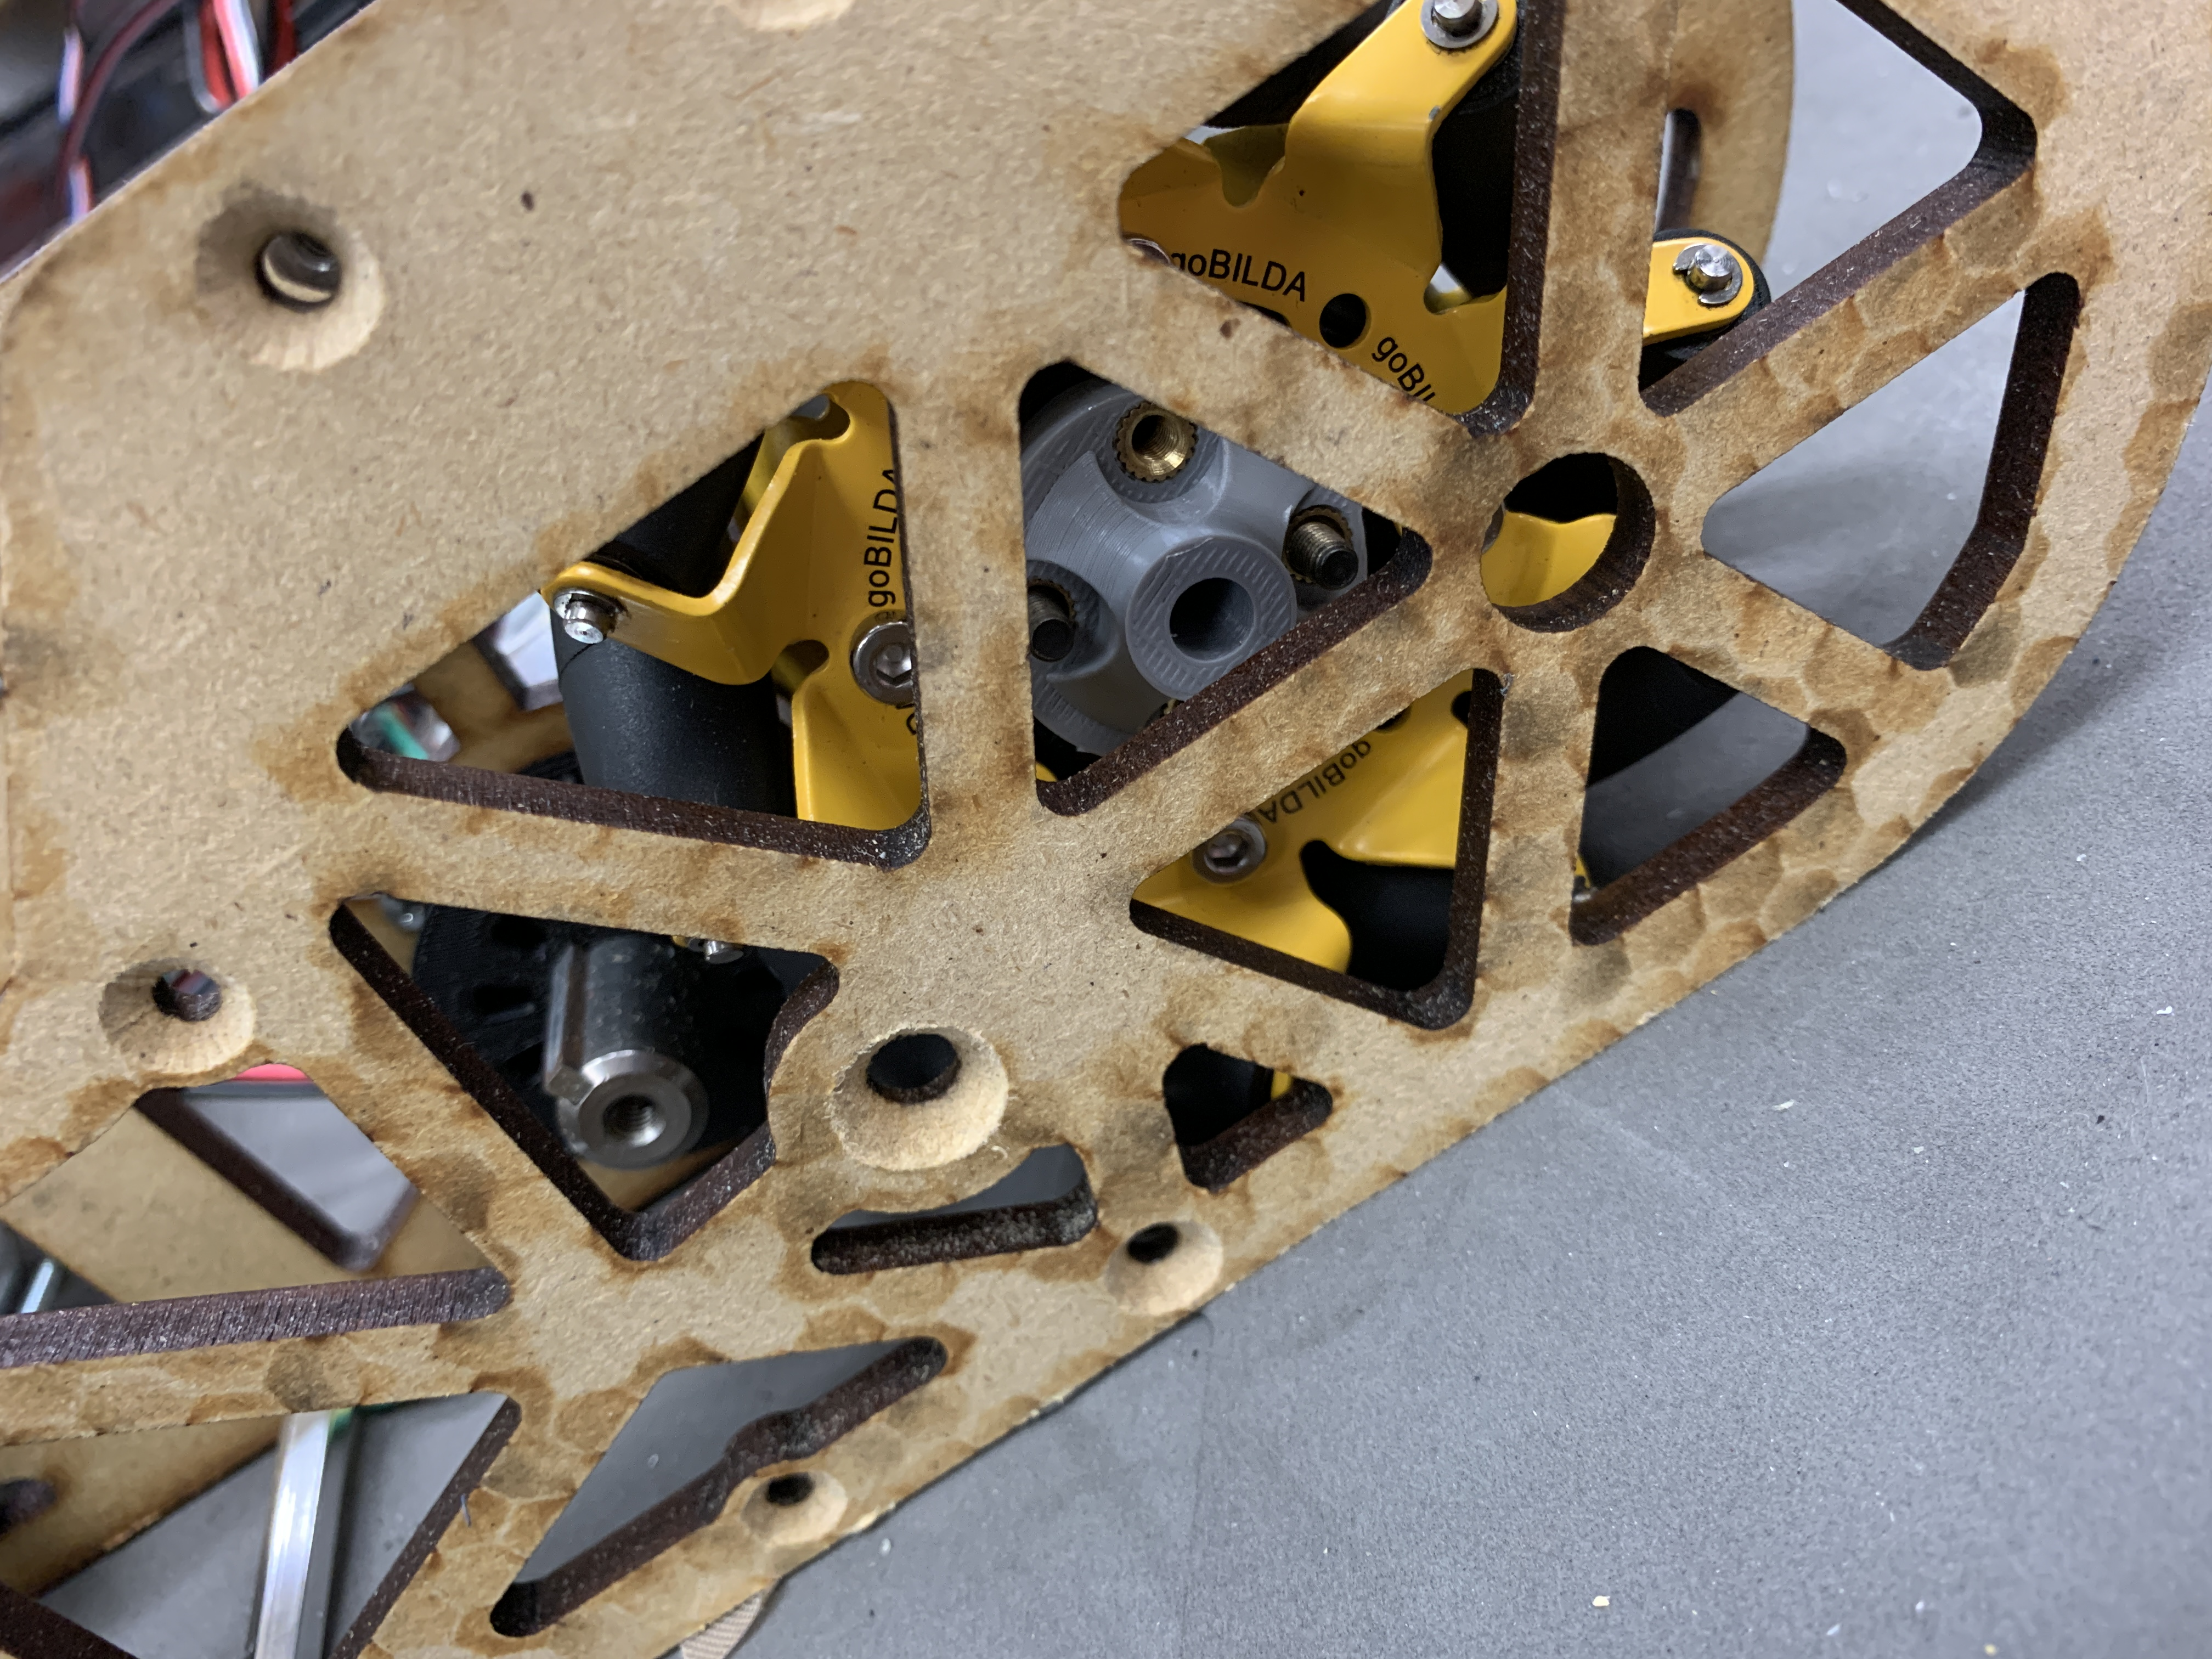
\includegraphics[width=0.8\textwidth]{Meetings/September/09-16-21/9-16-21_Hardware_Image2 - Nathan Forrer.JPG}
  \caption{The shafts that were falling out of the robot.}
  \label{fig:pic2}
\end{minipage}
\end{figure}

\begin{figure}[htp]
\centering
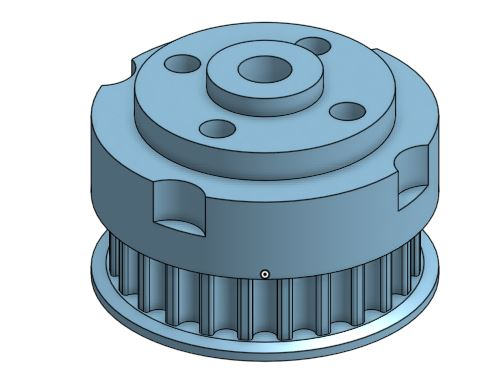
\includegraphics[width=0.9\textwidth, angle=0]{Meetings/September/09-16-21/9-16-21_Hardware_Image3 - Nathan Forrer.JPG}
\caption{This is the new CAD model for our wheel pulley.}
\label{fig:pic3}
\end{figure}

\subsection*{Software}
\noindent\hfil\rule{\textwidth}{.4pt}\hfil
\subsubsection*{Goals}
\begin{itemize}
    \item Fixing Arc Problem with Mecanum Drive

\end{itemize} 

\noindent\hfil\rule{\textwidth}{.4pt}\hfil

\subsubsection*{Accomplishments}
During this meeting, we continued to work on the tele op for the Mecanum Drive. We were aiming to get it done before the season so we didn't have to worry about it when the season started and we could do a lot of driver practice in advance. From last meeting, we continued to work on fixing the arc problem by using RUN USING ENCODER mode for the motors on the drivetrain. This would help maintain velocity on the motors, allowing them to strafe well. After some debugging and testing, we found out that the motors were so off from each other that they wouldn't be able to strafe even if we used RUN USING ENCODER mode. This problem may have came from incorrectly marking the gearboxes as 16:1's when they actually might have had a different gear ratio. For this reason, we will have to take apart the drivetrain and use the correct gearboxes on each motor.